\documentclass[12pt,a4paper]{article}
\usepackage{mathptmx} % added for time new roman font
\usepackage[left=0.5in,right=0.5in,top=1in,bottom=1in]{geometry}
\usepackage[latin1]{inputenc}
\usepackage{amsmath}
\usepackage{amsfonts}
\usepackage{amssymb}
\usepackage{graphicx}
\usepackage{float}
\usepackage{booktabs}
\usepackage{parskip} % remove all the paragraph indents


\usepackage{setspace}
\usepackage[colorlinks=true]{hyperref}
\usepackage{textcomp} 
\usepackage{multicol} 

\usepackage{mathtools}          %loads amsmath as well added for the piece wise function
\DeclarePairedDelimiter\Floor\lfloor\rfloor
\DeclarePairedDelimiter\Ceil\lceil\rceil

 
\newcounter{NumberInTable}
\newcommand{\LTNUM}{\stepcounter{NumberInTable}{(\theNumberInTable)}}

\newcommand{\Laplace}[1]{\ensuremath{\mathcal{L}{\left[#1\right]}}}
\newcommand{\InvLap}[1]{\ensuremath{\mathcal{L}^{-1}{\left[#1\right]}}}
\renewcommand{\textuparrow}{$\uparrow$}

\begin{document}
	
	\large{}
	\title{\vspace{-2cm}Lecture Notes, Topic-5}
	\date{}
	\maketitle
	
	\section*{Review from previous class}
	\begin{enumerate}
		\item Introduced the concept fo damping
		\item Modeled viscous damping in a 1 DOF system
	\end{enumerate}
	
	\section*{Objectives for today's class}
	\begin{enumerate}
		\item Introduce material stiffness and systems of springs. 
		\item Methods for measuring vibrating systems.
	\end{enumerate}
	
	\section*{Lecture}
	
		\subsection*{Stiffness}
			The stiffness, k, of a body is a measure of the resistance offered by an elastic body to deformation. For a single degree of freedom (DOF), the stiffness is defined as
			\begin{equation}
				k=\frac{F}{\delta}
			\end{equation}
			The stiffness of the spring that we have been considering can be more closely related to materials properties. Considering the following bar and mass:
			\begin{figure}[H]
				\centering
				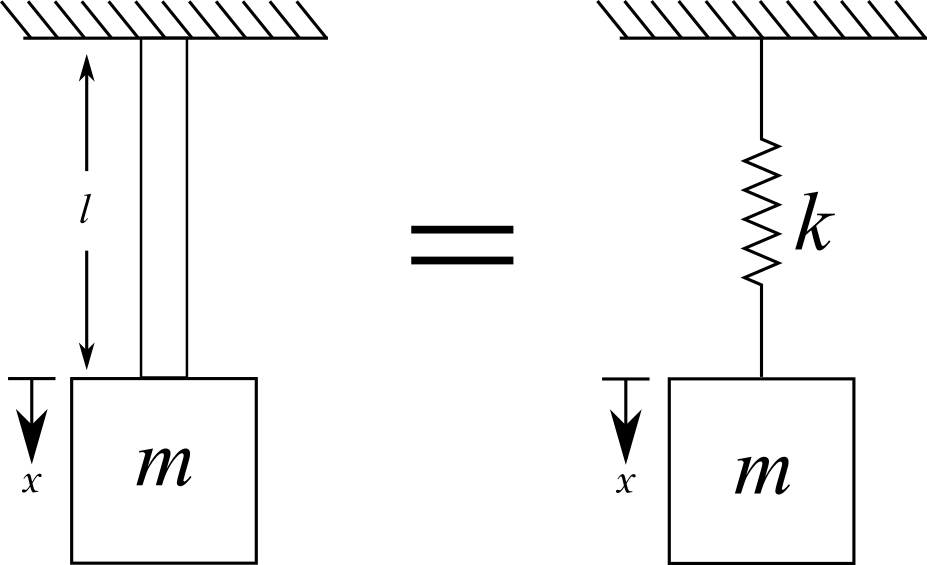
\includegraphics[width=0.5\textwidth]{../../Figures/spring_and_bar_mass_vertical.png}
			\end{figure}		
			From Hooke's law, we know that the force acting on a material can be expressed as 
			\begin{equation}
				f=EA
			\end{equation}
			 where $E$ is the elastic modulus and $A$ is the cross-sectional area of the beam. Now, let the deformation in the rod be defined as:
			\begin{equation}
				x=\Delta l
			\end{equation}			
			Next, $\Delta l$ can also be expressed as 
			\begin{equation}
				\delta = \Delta l = \frac{F l}{EA}
			\end{equation}				
			 we can combine this k=$\frac{F}{\delta}$ to get:
			\begin{equation}
				k = \frac{EA}{l}
			\end{equation}			
			In a similar fashion, we can also solve the equivalent system for a mass at the end of a cantilever beam.
			\begin{figure}[H]
				\centering
				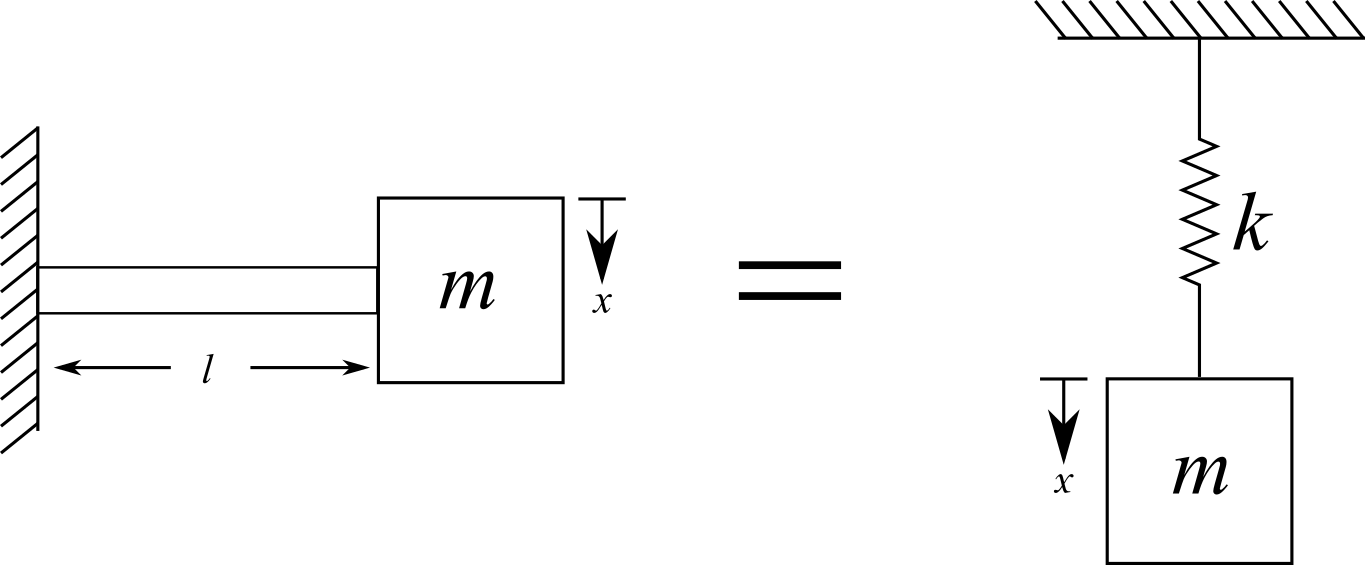
\includegraphics[width=0.7\textwidth]{../../Figures/spring_and_bar_mass_cantilever_beam.png}
			\end{figure}			
			From engineering mechanics we know that the deflection at the point of a beam $\delta$ of a beam with a point load $P$ is:
			\begin{equation}
				\delta = \frac{Pl^3}{3EI}
			\end{equation}					
			replacing the point load with a mass $mg$ and knowing that stiffness is $k=F/\delta$ we can show that  
			\begin{equation}
				k = \frac{3EI}{l^3}
			\end{equation}		

		\subsection*{Equivalent stiffness}						
			
			For systems with more than one spring acting on a body, equivalent stiffness can be calculated as

			\begin{figure}[H]
				\centering
				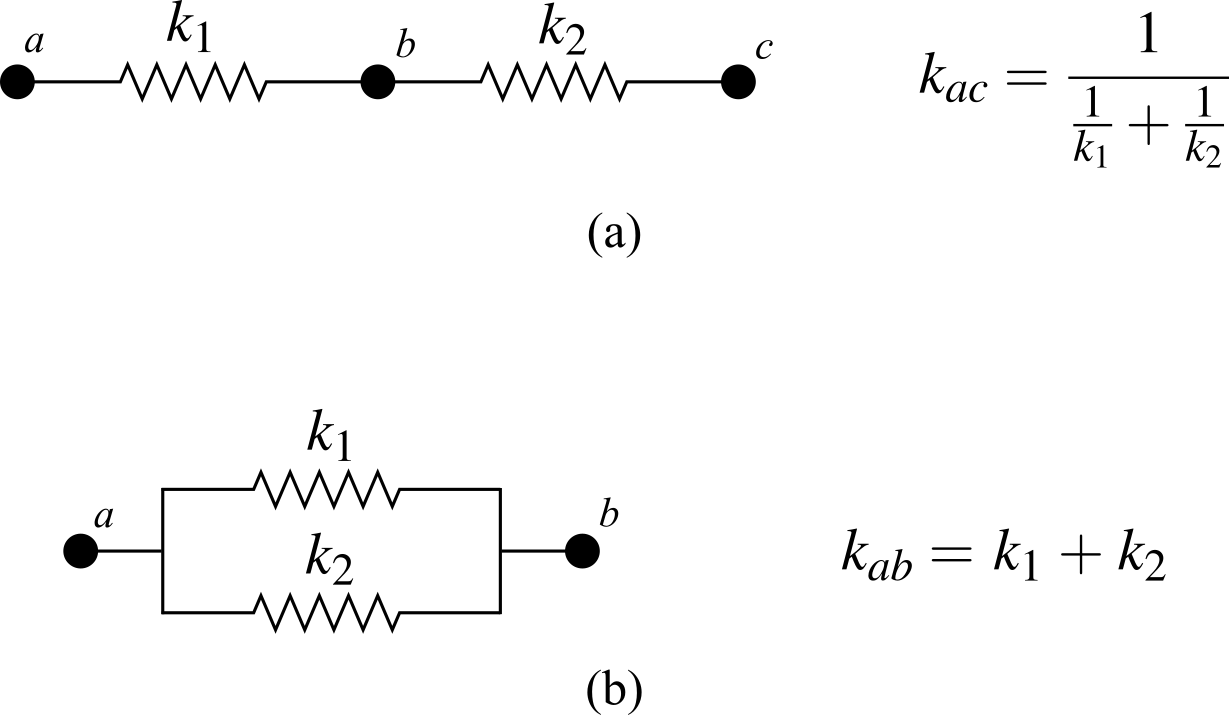
\includegraphics[width=0.5\textwidth]{../../Figures/equivalent_stiffness.png}
			\end{figure}	
			These are derived considering the displacement $\delta$ of the systems. For two springs in series:
			\begin{figure}[H]
				\centering
				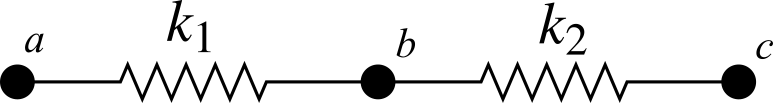
\includegraphics[width=0.3\textwidth]{../../Figures/equivalent_stiffness_series.png}
			\end{figure}			
			The total displacement is 
			\begin{equation}
				\delta_{ac} = \delta_{ab} + \delta_{bc}
			\end{equation}
			Using the equation for stiffness $k=F/\delta$, this converts to:
			\begin{equation}
				\frac{F}{k_{ac}} = \frac{F}{k_{1}} + \frac{F}{k_{2}}
			\end{equation}
			As $F$ is the same throughout the system, we can cancel out $F$. Solving for the equivalent stiffness yields:
			\begin{equation}
				k_{ac} = \frac{1}{\frac{1}{k_1}+\frac{1}{k_2}}
			\end{equation}
			Similarly for a system of springs in parallel:
			\begin{figure}[H]
				\centering
				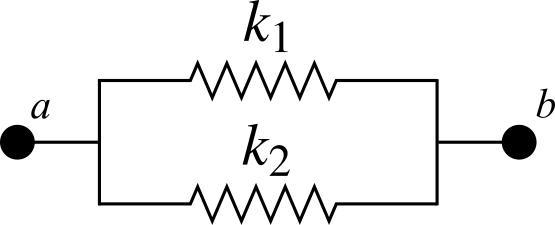
\includegraphics[width=0.2\textwidth]{../../Figures/equivalent_stiffness_parallel.png}
			\end{figure}			
			The displacement in both springs is the same, so the total displacement is 
			\begin{equation}
				\delta_{ab} = \delta_{\text{1}} =  \delta_{\text{2}} = \delta
			\end{equation}
			The forces in the direction of spring elongation sum to zero, therefore:
			\begin{equation}
				F_{ab} = F_{\text{1}} +  F_{\text{2}}
			\end{equation}			
			Substituting the displacement and stiffness into the force equation yields:
			\begin{equation}
				\delta k_{ab} = 	\delta k_{1} +  \delta k_{2}
			\end{equation}				
			this simplifies to:
			\begin{equation}
				k_{ab} = k_1+k_2
			\end{equation}

		\subsection*{Obtaining the damping coefficient of a system using the logarithmic decrement method}
		
			For a vibrating system, the  mass ($m$) and stiffness ($k$) can be measured using scales and static deflection tests. However, the damping coefficient ($c$) is a more difficult quantity to determine. From $k$ and $m$ we can compute the natural frequency ($\omega_n$) and the critical damping coefficient ($c_\text{cr}$). Therefore, knowing that the critical damping ratio ($\zeta$) is defined as:
			\begin{equation}
				\zeta = \frac{c}{c_{\text{cr}}} = \frac{c}{2\sqrt{km}} = \frac{c}{2m\omega_n}
			\end{equation}				
			if we calculate $\zeta$, we can obtain $c$ for the system of interest. This is made possible because $c_\text{cr}$ can be calculated from $k$ and $m$. Observing the temporal response for the underdamped system, 
			\begin{figure}[H]
				\centering
				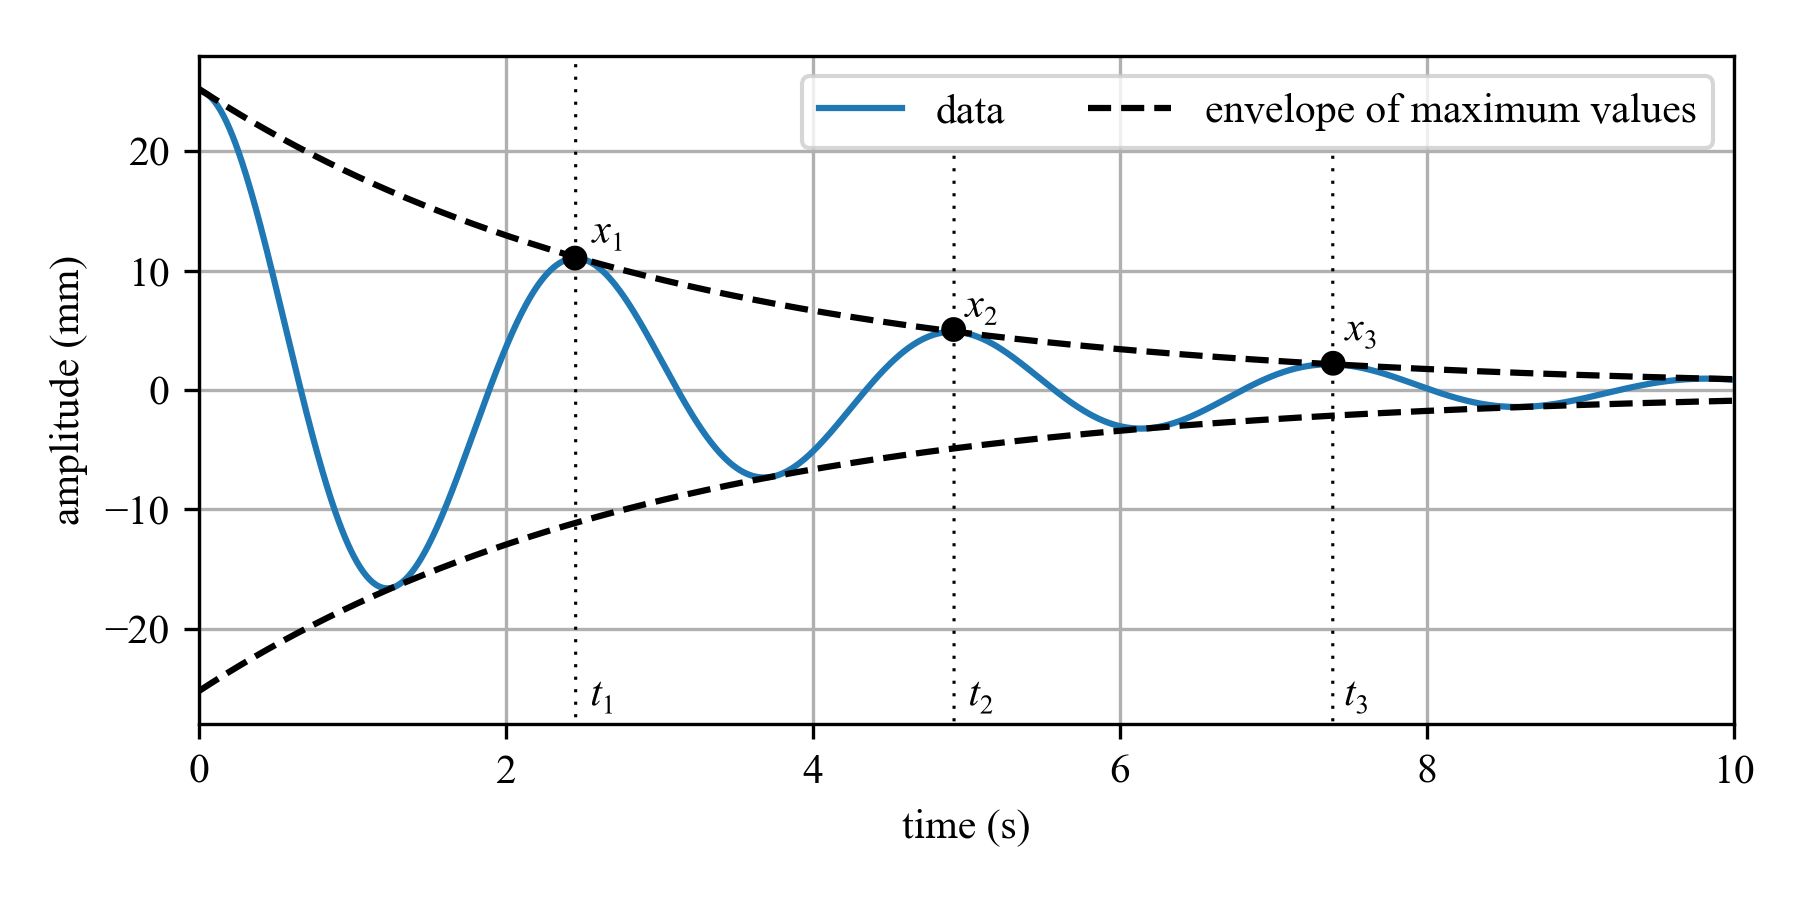
\includegraphics[width=0.9\textwidth]{../../Figures/Logarithmic_decrement.png}
			\end{figure}
			we mark three points of maximum amplitude, $x_1$, $x_2$, and $x_3$ that happen at $t_1$, $t_2$, and $t_3$, respectively. Considering displacement values for the first two points $x_1$ and $x_2$. separated by a complete period ($T$).  Knowing that one cycle is $2 \pi$, the time period for this complete cycle is given by:
			\begin{equation}
				t_2-t_1 = \frac{2\pi}{\omega_d} = \frac{2\pi}{\sqrt{1-\zeta^2}\omega_n}
			\end{equation}				
			where $\omega_d$ is the damped natural frequency. This is the time period ($T$) of damped oscillations. If derive an equation for the values of the peaks, also called the envelope of maximum values, we get: 
			\begin{equation}
				x_{\text{peaks}} = Ae^{-\zeta\omega_nt} 
			\end{equation} 		
			Knowing that the system is underdamped, $A$ can be solved for using the initial conditions $x_0$ and $v_0$, therefore: 
			\begin{equation}
				A = \frac{\sqrt{(v_0+\zeta\omega_nx_0)^2 + (x_0\omega_d)^2}}{\omega_d}
			\end{equation} 	
			In terms of $t_1$ and $t_2$, we can express the displacement at these times as:
			\begin{equation}
				x_{\text{1}} = A e^{-\zeta \omega_n t_1}
			\end{equation}				
			and 
			\begin{equation}
				x_{\text{2}} = A e^{-\zeta \omega_n t_2}
			\end{equation}		
			therefore:
			\begin{equation}
				\frac{x_{\text{1}}}{x_{\text{2}}} = e^{\zeta \omega_n(t_2-t_1)}
			\end{equation}		
			However, from before we know that $t_2-t_1 = \frac{2\pi}{\sqrt{1-\zeta^2}\omega_n}$. Therefore, we can express this last equation as:
			\begin{equation}
				\frac{x_{\text{1}}}{x_{\text{2}}} =e^{\Big(\frac{2 \pi \zeta}{\sqrt{1-\zeta^2}}\Big)}
			\end{equation}			
			Next, we take the natural log of both sides to get the \textbf{logarithmic decrement}, denoted by $\delta$:
			\begin{equation}
				\delta = \text{ln}\bigg(\frac{x_{\text{1}}}{x_{\text{2}}}\bigg) = \text{ln}\bigg(\frac{x(t_{\text{1}})}{x(t_{\text{1}}+T)}\bigg) = \frac{2 \pi \zeta}{\sqrt{1-\zeta^2}}
			\end{equation}				
			This shows us that the ratio of any two successive amplitudes for an underdamped system, vibrating freely, is constant and is a function of the damping only. Sometimes, in experiments, it is more convenient/accurate to measure the amplitudes after say ``$n$'' peaks rather than two successive peaks (because if the damping is very small, the difference between the successive
			peaks may not be significant). The logarithmic decrement can then be given by the equation
			\begin{equation}
				\delta = \frac{1}{n}\text{ln}\bigg(\frac{x_{\text{1}}}{x_{\text{n+1}}}\bigg) =   \frac{1}{n}\text{ln}\bigg(\frac{x(t_{\text{1}})}{x(t_{\text{1}}+nT)}\bigg) = \frac{2 \pi \zeta}{\sqrt{1-\zeta^2}}
			\end{equation}				
			Once we use the experimental data to obtain $\delta$, and knowing that:
			\begin{equation}
				\delta = \frac{2 \pi \zeta}{\sqrt{1-\zeta^2}}
			\end{equation}	
			we can calculate the value of $\zeta$:
			\begin{equation}
				\zeta = \frac{\delta}{\sqrt{4\pi^2+\delta^2}}
			\end{equation}
			Therefore, having $\zeta$ we can solve for the coefficient of damping, $c$, as: 
			\begin{equation}
				c = \zeta 2\sqrt{km}
			\end{equation}					
			
		\subsection*{Example 1}
			Calculate the damping coefficient of the problem expressed above given that $m$ = 3 kg and $k$ = 20 N/m, $x_1$ = 11 mm, and $x_3$ = 2 mm.
			
			First, we solve for $\delta$, for $n$ = 2:  
			\begin{equation}
				\delta = \frac{1}{2}\text{ln}\bigg(\frac{x_{\text{1}}}{x_{\text{3}}}\bigg) = \frac{1}{2}\text{ln}\bigg(\frac{11.03}{2.15}\bigg) = 0.852
			\end{equation}						
			Next, we can calculate $\zeta$, as: 
			\begin{equation}
				\zeta = \frac{\delta}{\sqrt{4\pi^2+\delta^2}} = \frac{0.817}{\sqrt{4\pi^2+0.817^2}} = 0.134
			\end{equation}
			And lastly:			
			\begin{equation}
				c = \zeta 2\sqrt{km} = 0.134 \cdot 2\sqrt{20 \cdot 3} = 2.08 \text{ kg/s}
			\end{equation}	
			
		\subsection*{Example 2} 
			The free response of a 1000-kg automobile with a stiffness of $k$ = 400,000 N/m is observed to be underdamped. Modeling the automobile as a single-degree-of-freedom oscillation in the vertical direction, determine the damping coefficient if the displacement at $t_1$ is measured to be 2 cm and 0.22 cm at $t_2$.
			
			Knowing $x_1$ = 2 cm and $x_2$ = 0.22 cm and $t_2 = T + t_1$, therefore:
			\begin{equation}
				\delta = \text{ln}\frac{x_1}{x_2} = \text{ln}\frac{2}{0.22} = 2.207
			\end{equation}			
			and:
			\begin{equation}
				\zeta = \bigg(\frac{\delta}{\sqrt{4\pi^2+\delta^2}}\bigg) = \bigg(\frac{2.207}{\sqrt{4\pi^2+2.207^2}}\bigg) = 0.331
			\end{equation}
			therefore, we can obtain the damping coefficient as
			\begin{equation}
				c = 2\zeta\sqrt{km}=2(0.331)\sqrt{400,000 \cdot 1,000} = 13,256 \hspace{1ex} 
				\text{kg/s} 
			\end{equation}	
		
		\subsection*{Example 3}
			Calculate the undamped frequency of the following system:
			\begin{figure}[H]
				\centering
				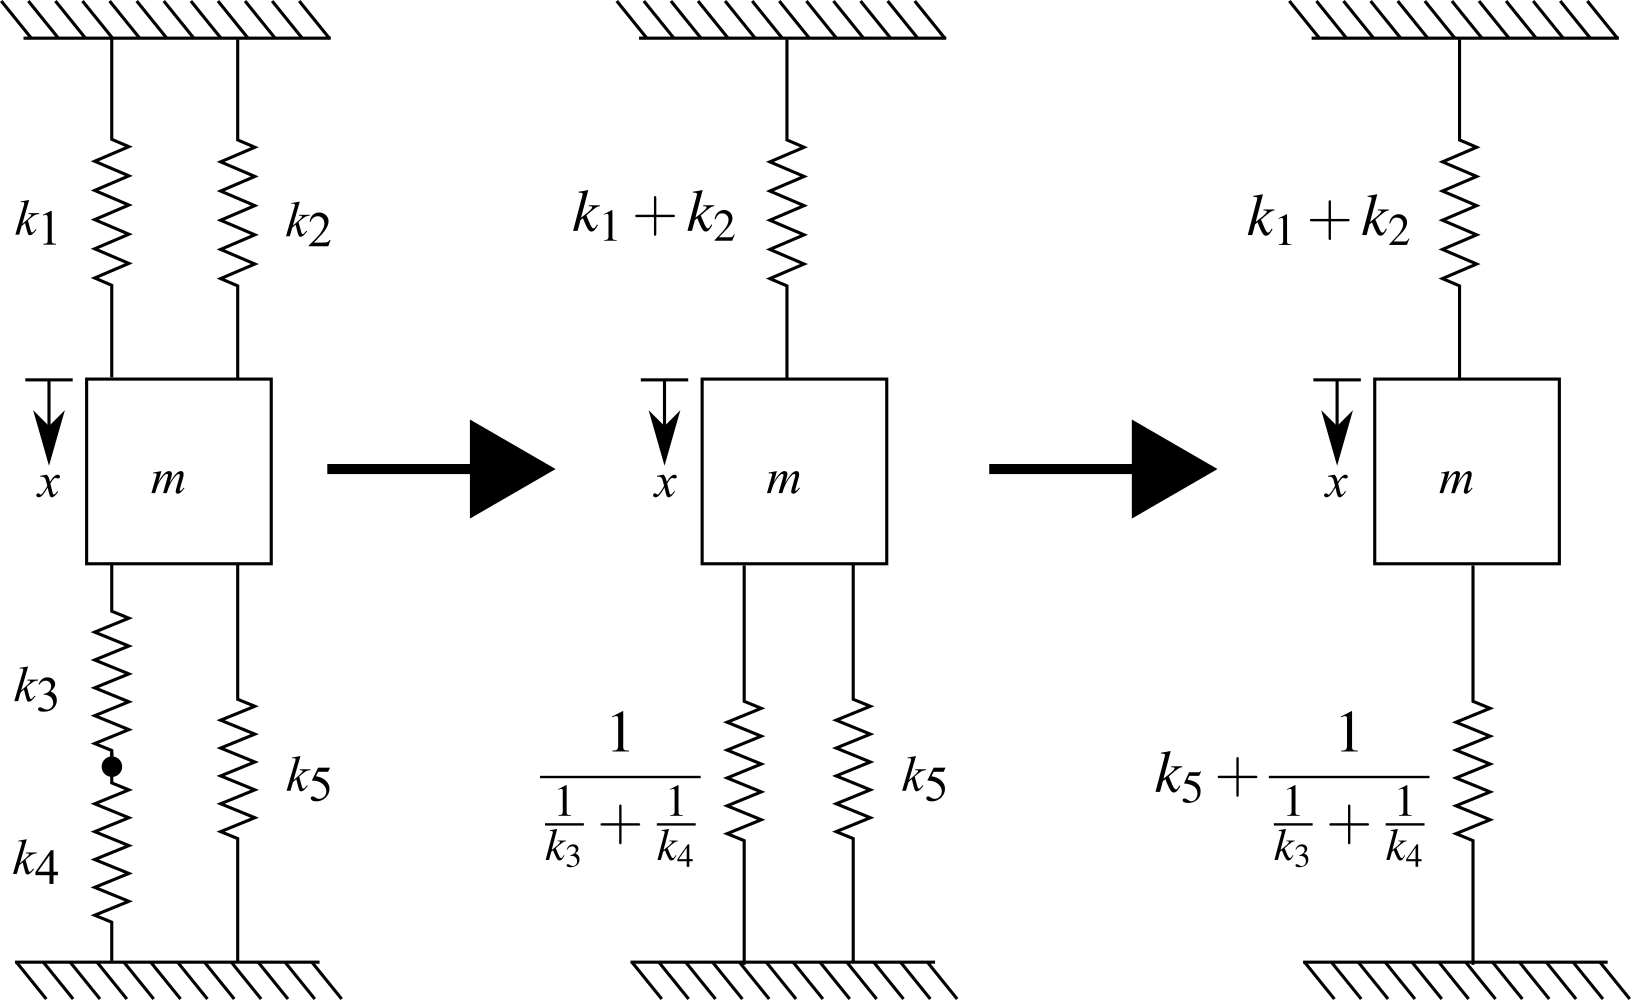
\includegraphics[width=0.7\textwidth]{../../Figures/equivalent_mass_and_spring_system_1.png}
			\end{figure}	
			The springs are combined as shown, using the equations defined before.  Now, considering that the displacement ($\delta$) of the top spring, and the bottom spring are the same we can state the total stiffness $k$, is the summation of the two. Therefore,    
			\begin{figure}[H]
				\centering
				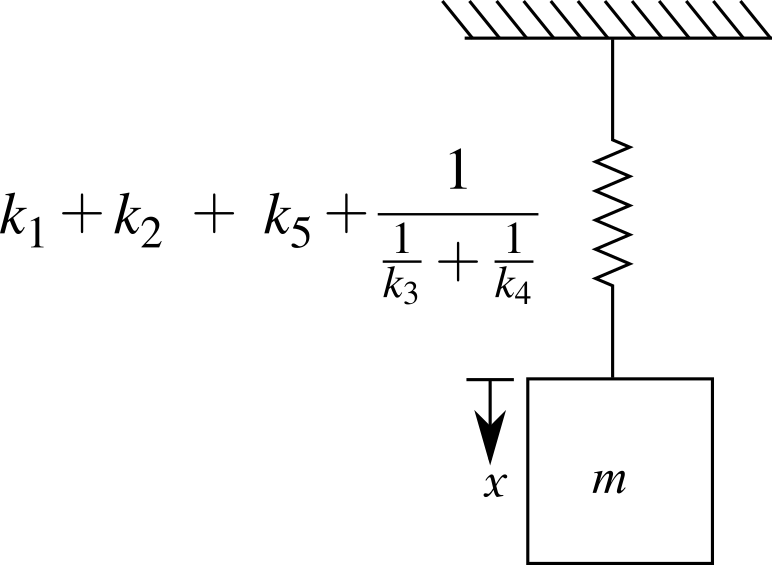
\includegraphics[width=0.3\textwidth]{../../Figures/equivalent_mass_and_spring_system_2.png}
			\end{figure}	
%			until a final $k$ value can be obtained:
%			\begin{equation}
%				k=k_1+k_2+k_5+\frac{1}{\frac{1}{k_3}+\frac{1}{k_4}}
%			\end{equation}		
			rearranging to get a common denominator:
			\begin{equation}
				k= \frac{(k_1+k_2+k_5)(k_3+k_4)+k_3k_4}{k_3+k_4}  
			\end{equation}				
			For an arbitrary mass, $m$, the undamped frequency $\omega_n$ can be calculated as:
			\begin{equation}
				\omega_n = \sqrt{\frac{k}{m}} = \sqrt{\frac{(k_1+k_2+k_5)(k_3+k_4)+k_3k_4}{m(k_3+k_4)} }
			\end{equation}				

	 
			
			
\end{document}